\begin{figure}[h]
    \centering
    \begin{subfigure}{.5\textwidth}
      \centering
      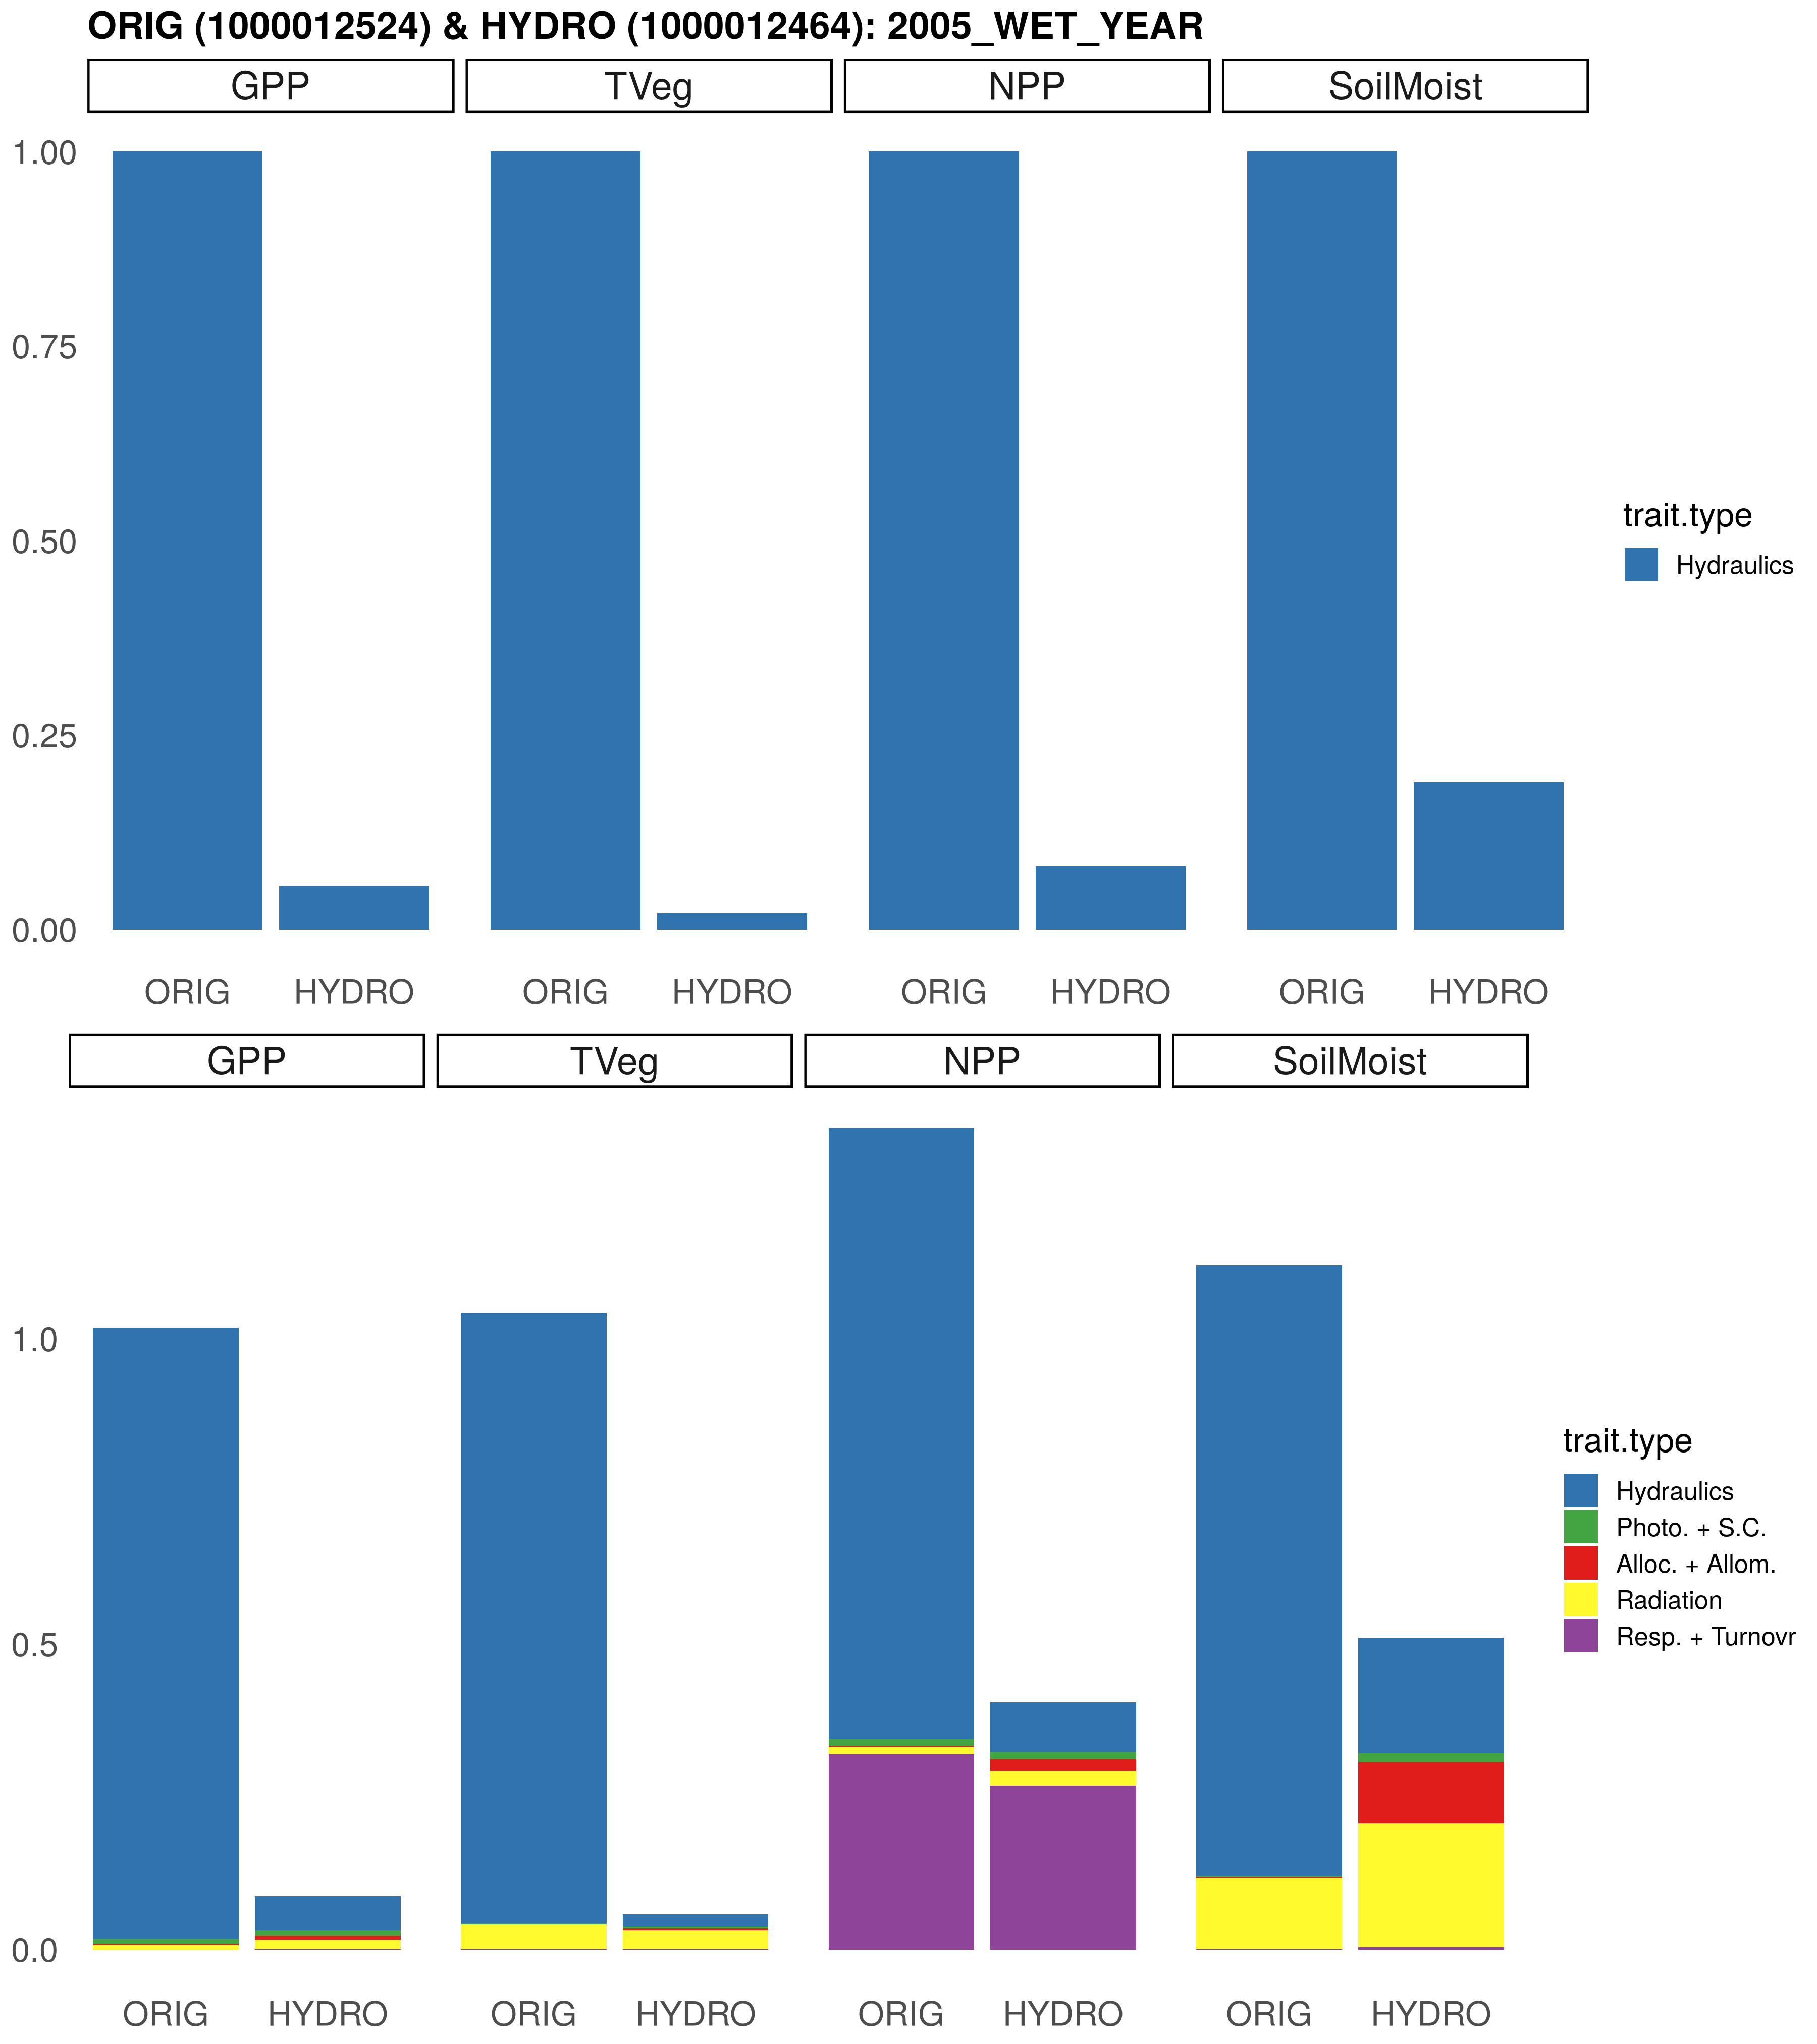
\includegraphics[width=.95\linewidth]{Hydro_Paper_LaTeX/Hydro_Paper_Figures/barplot_wet_year.png}
      \caption{Wet year}
      \label{fig:barplot_wet}
    \end{subfigure}%
    \begin{subfigure}{.5\textwidth}
      \centering
      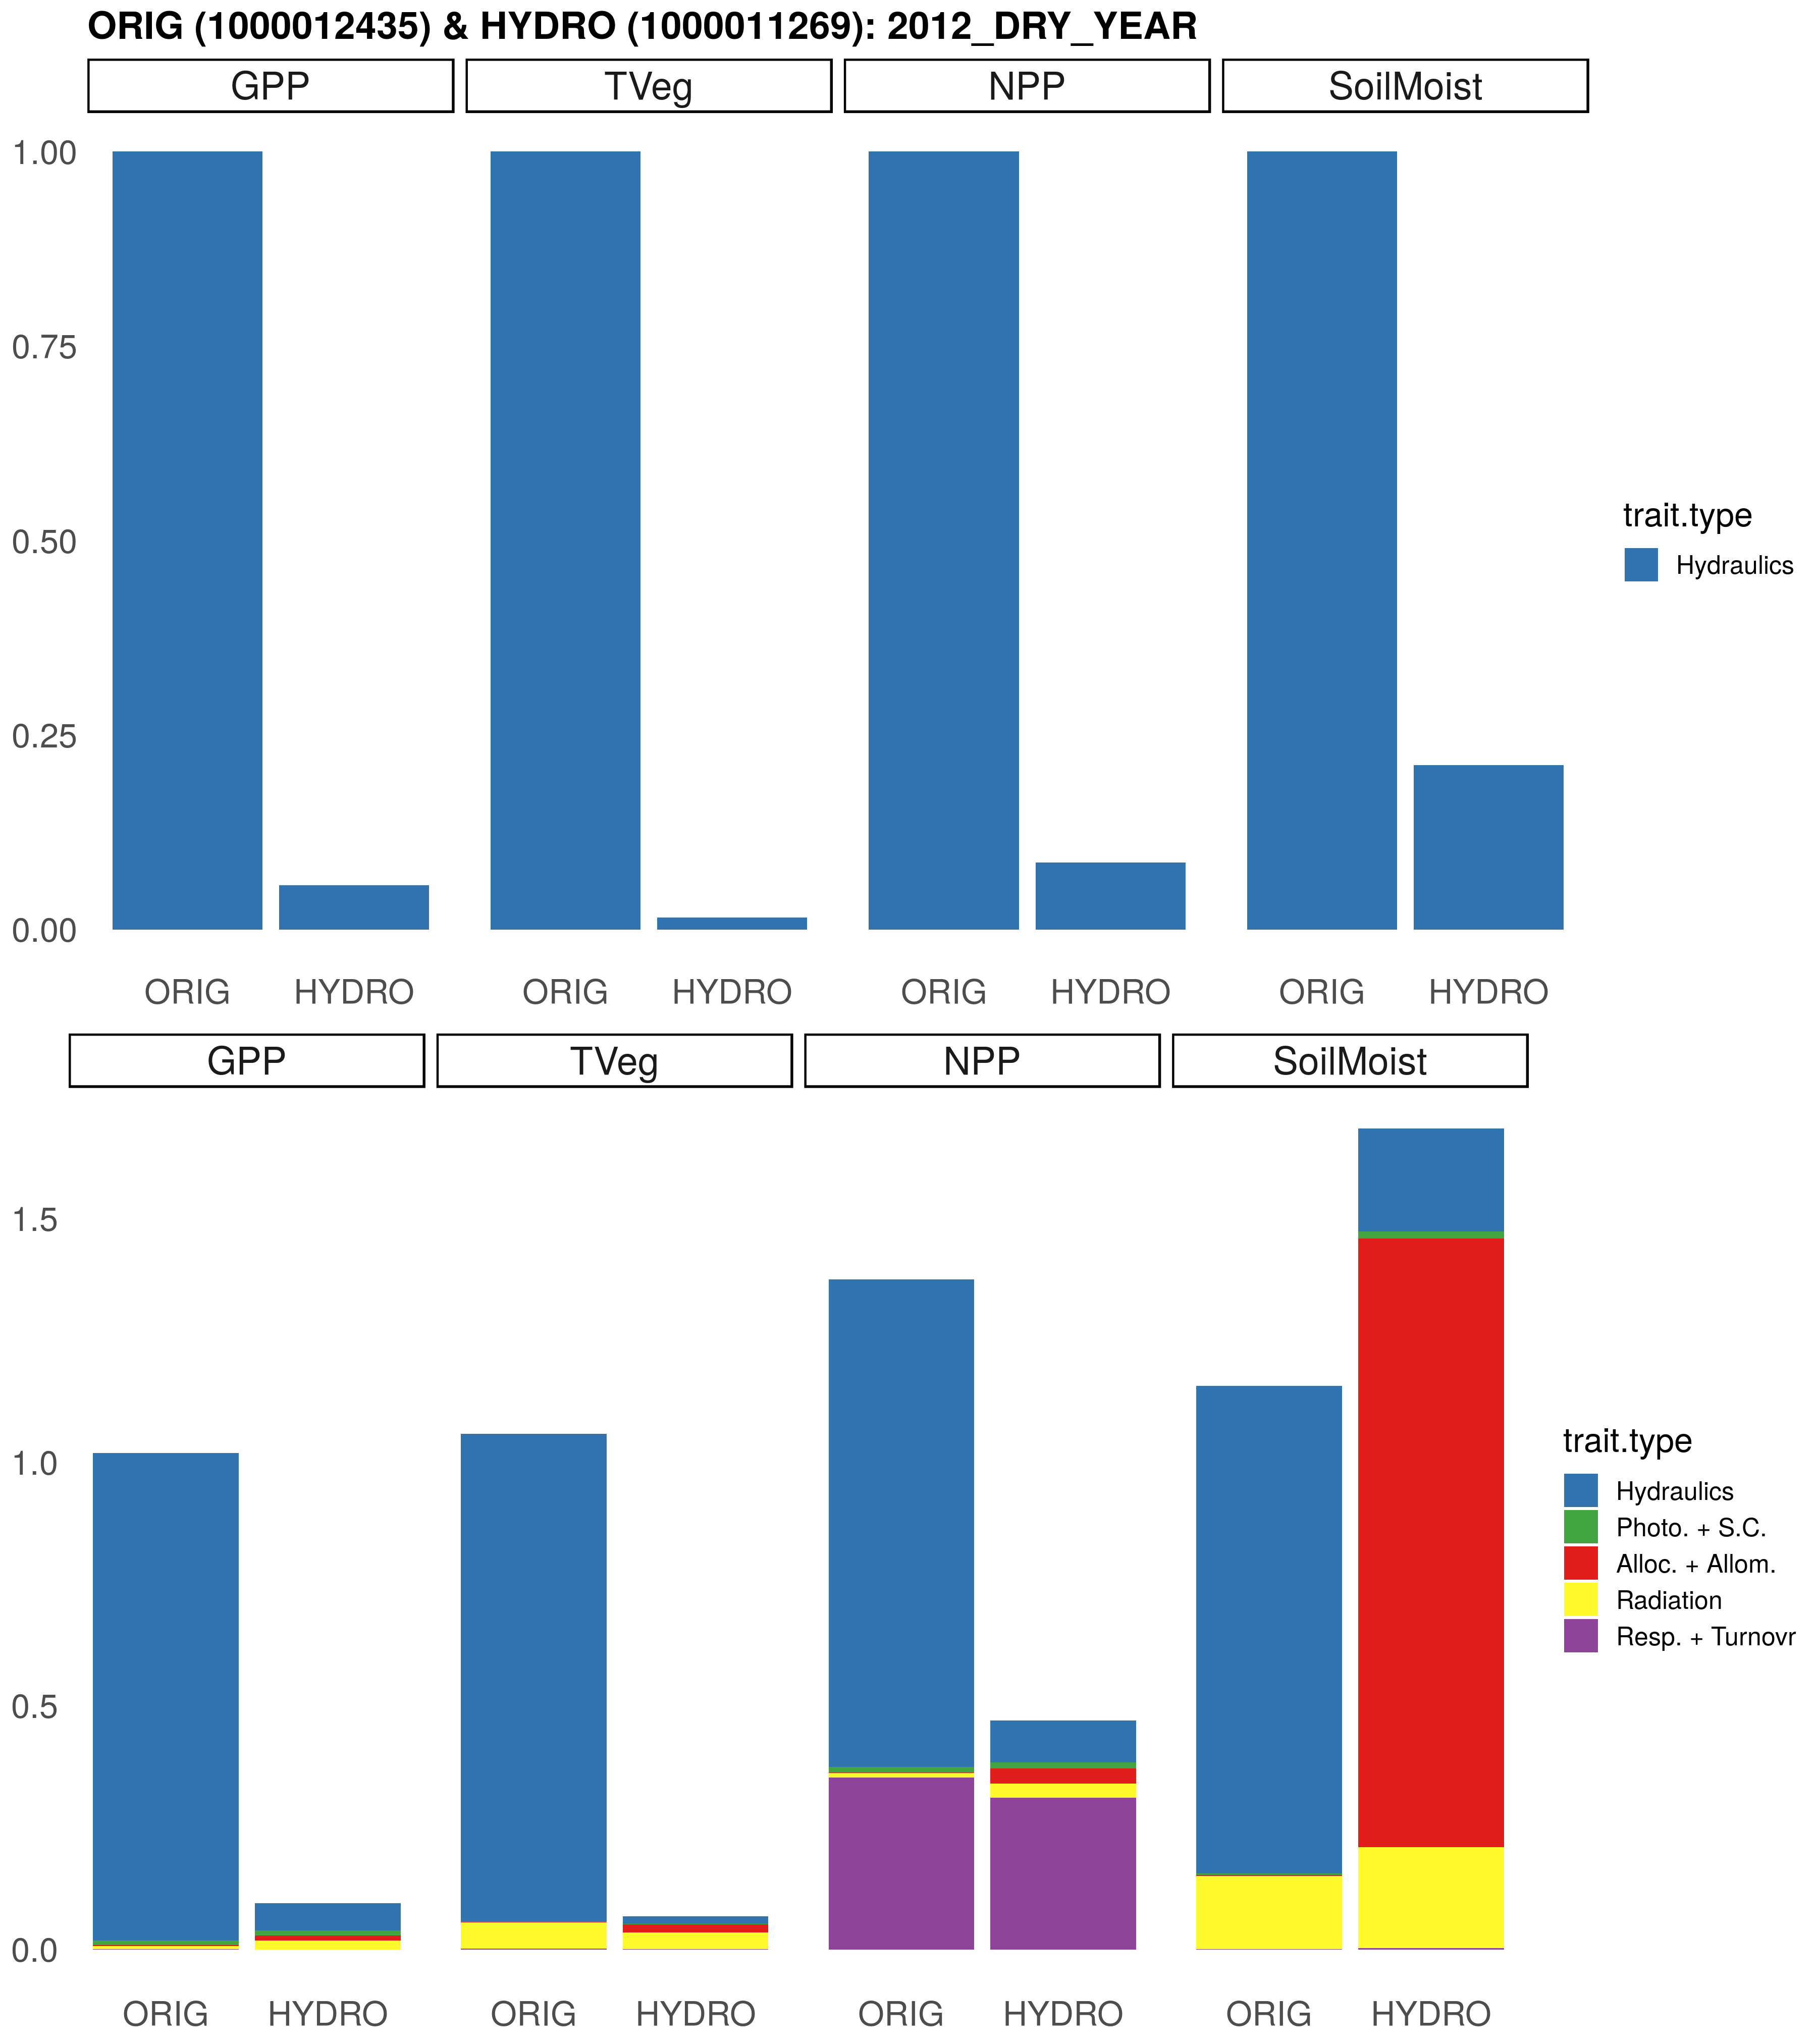
\includegraphics[width=.95\linewidth]{Hydro_Paper_LaTeX/Hydro_Paper_Figures/barplot_dry_year.png}
      \caption{Dry year}
      \label{fig:barplot_dry}
    \end{subfigure}
    \caption{Barplots of wet and dry years. Blue is hydro, red is allocation. The other colors are other things. \\
    \\
    Current feedback on the figure includes:\\
    - The colors need to change because they are ugly\\
    - All everything is too small and hard to read. \\
    - "TVeg" should be changed to something more intuitive like "Transp."
    }
    \label{fig:test}
\end{figure}